\documentclass[review]{elsarticle}

\usepackage{amsmath}
\usepackage{amssymb}
\usepackage{lineno,hyperref}
\usepackage{subcaption} 
\usepackage{booktabs}
\usepackage{multirow}
\graphicspath{{./figures/}}
\modulolinenumbers[5]
\DeclareMathOperator*{\argmin}{arg\,min}
\newcommand{\angstrom}{\text{\normalfont\AA}}
\journal{XXX}

%%%%%%%%%%%%%%%%%%%%%%%
%% Elsevier bibliography styles
%%%%%%%%%%%%%%%%%%%%%%%
%% To change the style, put a % in front of the second line of the current style and
%% remove the % from the second line of the style you would like to use.
%%%%%%%%%%%%%%%%%%%%%%%

%% Numbered
%\bibliographystyle{model1-num-names}

%% Numbered without titles
%\bibliographystyle{model1a-num-names}

%% Harvard
%\bibliographystyle{model2-names.bst}\biboptions{authoryear}

%% Vancouver numbered
%\usepackage{numcompress}\bibliographystyle{model3-num-names}

%% Vancouver name/year
%\usepackage{numcompress}\bibliographystyle{model4-names}\biboptions{authoryear}

%% APA style
%\bibliographystyle{model5-names}\biboptions{authoryear}

%% AMA style
%\usepackage{numcompress}\bibliographystyle{model6-num-names}

%% `Elsevier LaTeX' style
\bibliographystyle{elsarticle-num}
%%%%%%%%%%%%%%%%%%%%%%%

\begin{document}

\begin{frontmatter}

\title{Radiation Damage in Polyatomic Materials using Damage Energy Functions}
%\title{Radiation Damage\tnoteref{mytitlenote}}
%\tnotetext[mytitlenote]{INL Internship Summer 2017}

%% Group authors per affiliation:
\author{Sebastian Schunert, Daniel Schwen}
\address{Fuels Modeling and Simulation Department, Idaho National Laboratory, P.O Box 1625, Idaho Falls, ID 83415}
%\fntext[myfootnote]{Since 1880.}

%% or include affiliations in footnotes:
%\author[mymainaddress,mysecondaryaddress]{Elsevier Inc}
%\ead[url]{www.elsevier.com}

%\author[mysecondaryaddress]{Global Customer Service\corref{mycorrespondingauthor}}
%\cortext[mycorrespondingauthor]{Corresponding author}
%\ead{support@elsevier.com}

%\address[mymainaddress]{1600 John F Kennedy Boulevard, Philadelphia}
%\address[mysecondaryaddress]{360 Park Avenue South, New York}

\begin{abstract}

\end{abstract}

\begin{keyword}
Radiation damage\sep  \sep Inelastic scattering
%\MSC[2010] 00-01\sep  99-00
\end{keyword}

\end{frontmatter}

\linenumbers

\section{Introduction}
The number of displacements caused by a primary knock-on atom (PKA) of given energy is of central importance for predicting the evolution of the material properties in the presence of irradiation. 
The binary-collision Monte-Carlo (BCMC) method~\cite{SRIM} can be used to simulate representative radiation damage cascades caused by an atom of given type, $(Z, A)$ numbers, and initial energy. The \textit{SRIM} code~\cite{SRIM} allows computation of spatial distributions of point defects in one-dimensional geometries for polyatomic, amorphous materials. The \textit{mytrim}~\cite{Schwen2010} code allows BCMC simulations in general three-dimensional geometries.  
In this report, we focus on a zero-dimensional representation of the average displacement rate. This approach is intended for improving the 
efficiency of coupled FEM-BCMC calculations as implemented in the \textit{Mesoscale Atomistic Glue Program for Integrated Execution (Magpie)} that coupled MOOSE~\cite{Derek2015} based FEM applications with the \textit{mytrim} code. During these calculations, averaged point defect density rates in FEM mesh elements are computed setting the required resolution to roughly $h_{max}$ defined as the maximum mesh spacing. Lower energy knock-on atoms may create cascades that are fully encompassed within a single or very few mesh elements. Therefore, the ultimate benefit of following the cascade to its termination is limited, but requires significant computational resources. We propose to only follow knock-ons above a threshold energy explicitly by BCMC and use a zero-dimensional model for estimating the displacement rates below this threshold. 

In mono-atomic materials Kinchin and Pease's work~\cite{Kinchin1955} allows the computation of the number of displacements  
produced by a collision cascade of hard sphere. Subsequent work refining some assumptions but still limited to mono-atomic materials are
summarized in~\cite{GaryWas}.

In polyatomic materials Parkin and Coulter state integrodifferential equations for the total and net displacement rates~\cite{PC1981} that ultimately go back to work by Lindhard et al.~\cite{Lindhard1963}. The total and net displacement rates functions of the PKA energy only, i.e. they are not functions of space, and the integrodifferential equations contain both derivatives and integrals with respect to energy. Later, Huang and Ghoniem~\cite{Huang1993} used a slightly modified set of equations for the total displacement rate for computing neutron displacement damage cross sections for SiC.

In this work, we first introduce the equations for total and net displacement rate given by Parkin and Coulter~\cite{PC1981} and then 
relate them to the slightly simpler equations in the work of Huang and Ghoniem~\cite{Huang1993}. The final set of equations that will be numerically approximated in the \textit{Magpie} code will be presented along with the explicit form of the collision cross section. Numerical algorithms will be developed to solve the set of integrodifferential equations.

\section{Damage Energy, Total and Net Displacement Functions}
The damage energy function $nu_i(E)$ is defined as the energy that a projectile of type $i$ deposits as damage energy, i.e. energy that is imparted in follow-on knock-on atoms, in the material~\cite{PC1980} as opposed to dissipating it as heat. Nuclear collisions lead to the creation of secondary knock-ons while electronic stopping dissipates energy as heat and does not cause secondary displaced atoms. Damage energy is governed by the following set if integro-differential equations~\cite{PC1980}:
\begin{equation}\label{eq:damage_energy_function_1}
   S_i(E) \frac{d \nu_i}{dE} = \sum\limits_{k=1}^K   \frac{N_k}{N} \int\limits_{0}^{\Lambda_{ik} E}  \frac{d \sigma_{ik} (E,T)}{dT}  
   \left( \nu_k(T) + \nu_i(E-T) - \nu_i(E) \right) dT,
\end{equation}
where $S_i(E) = N \left(\frac{dE}{dx}\right)_i$ is the electronic stopping cross section of species $i$ moving with energy $E$, $N_k$ is the number density of species $k$, $N$ is the total number density of the background material, $\Lambda_{ik} = \frac{4A_i A_j}{(A_i + A_j)^2}$, $\frac{d \sigma_{ik} (E,T)}{dT}$ is the differential scattering cross section for interaction of species $i$ and $k$ ($i$: projectile, $k$ target). The initial conditions are given by Ref. ~\cite{Lindhard1963} as:
\begin{equation}\label{eq:damage_energy_function_2}
   \lim\limits_{E \rightarrow 0} \frac{\nu_i}{E} = 1.
\end{equation}
It is noted that conservation of energy requires that $\nu_i(E) \le E$ and consequently the limit in Eq.~\ref{eq:damage_energy_function_2} is approached from below. It is useful to define a damage energy efficiency $\eta_i = \nu_i / E$ that naturally varies between $0$ and $1$.

The total displacement function $\nu_{ij}(E)$ is the average number of atoms of type $j$ being displaced at least during a portion of the cascade by an atom of type $i$ and energy $E$. The displacement function $\nu_{ij}(E)$ counts the PKA itself. For convenience we define the total displacement function $n_{ij} = \nu_{ij} - \delta_{ij}$ that excludes the PKA. In contrast, the net displacement rate $g_{ij}(E)$ is defined as the number of atoms of type $j$ displaced and not recaptured by PKA of type $i$ and energy $E$~\cite{PC1981}. The set of integrodifferential equations governing the total displacement rate $\nu_{ij}$ is given by:
\begin{align}\label{eq:total_pc_1}
  S_{i}(E) \frac{d n_{ij}}{dE}  &= \sum\limits_{k=1}^K   \left[ \frac{N_k}{N} \int\limits_{0}^{\Lambda_{ik}E} dT \frac{d \sigma_{ik} (E,T)}{dT} \right . 
  \times \left \{   \rho_k(T) \left[  \delta_{k,j} + n_{kj}(T-E_k^b) \right] \right .
  \nonumber \\
  &+ \left . \left .  \left( 1 - \rho_k(T) \lambda_{ik}(E-T) \right)n_{ij}(E-T)  -n_{ij}(E)\right \} \right],
\end{align}
 where $\delta_{k,j}$ is the Kronecker delta, $E_k^b$ is the binding energy defined as the energy that an atom of type $k$ loses to inelastic processes and lattice vibrations as it is displaced from its lattice position, and:
\begin{align}
 \rho_k(T) &= \left\{ \begin{array}{ll}
         0, & ~ T < E_k^d\\
         1, & ~ T \ge E_k^d \end{array} \right.  \nonumber \\
 \lambda_{ik}(E) &=  \left\{ \begin{array}{ll}
         1, & ~ T < E_{ik}^{\text{cap}}\\
         0, & ~ T \ge E_{ik}^{\text{cap}} ,\end{array} \right.  
\end{align} 
where $E_k^d$ is the displacement threshold for species $k$ and $E_{ik}^{\text{cap}}$ is the residual energy threshold of an atom of type $i$ which has displaced an atom of type $k$ to be trapped in the vacant $k$ site. Intial conditions are provided by~\cite{PC1981} as $n_{ij} = 0 ~\text{for} ~E < \min\limits_{i} E_i^d$. For integration of Eq.~\ref{eq:total_pc_1} it is convenient to convert $\rho_k$ and $\lambda_{ik}$ into integration limits:
\begin{align}\label{eq:total_pc_2}
  S_{i}(E) &\frac{d n_{ij}}{dE}  = \sum\limits_{k=1}^K \frac{N_k}{N}   \left[ \int\limits_{E_k^d}^{\Lambda_{ik}E}  \frac{d \sigma_{ik} (E,T)}{dT}
  \left(  \delta_{k,j} + n_{kj}(T-E_k^b) \right) dT
    \right . \nonumber \\
    & \left . +\int\limits_{0}^{\Gamma_{ik}(E)}  \frac{d \sigma_{ik} (E,T)}{dT}  n_{ij}(E-T) dT +n_{ij}(E) \int\limits_{0}^{\Lambda_{ik}E}  \frac{d \sigma_{ik} (E,T)}{dT}   dT \right ] ,
\end{align}
where $\Gamma_{ik}(E)$ will be defined shortly. We note that $1 - \rho_k(T) \lambda_{ik}(E-T)$ is zero if both $\rho_k$ and $\lambda_{ik}$ are equal to one, otherwise the expression evaluates to one. For the expression to be zero, we obtain the conditions $T > E_k^d$ and $T > E - E_{ik}^{\text{cap}}$. Hence, we can determine $\Gamma_{ik}(E)$ to be
\[
\Gamma_{ik}(E) = \min \left( \Lambda_{ik} E, \max \left( E_k^d, E - E_{ik}^{\text{cap}} \right)  \right).
\]
The integrals in Eq.~\ref{eq:total_pc_2} will be referred to as integals (i), (ii), and (iii).
Several differences between the integrodifferential equations in Ref.~\cite{Huang1993} and Eq.~\ref{eq:total_pc_2} are noteworthy. First,
the upper limit of integral (ii) in~\cite{Huang1993} is given by $\min \left( \Lambda_{ik} E, E - E_{j}^d / \Lambda_{ij}  \right)$ as opposed to $\Gamma_{ik}$ [need to answer the question what the default value for $E_{ik}^{\text{cap}}$ should be. In HG, the $i,j$ index makes no apparent sense and I might have implemented incorrectly right now.]. Second, the argument of $n_{k,j}$ in integral (i) does not contain the binding energy. While the original derivation of Lindard~\cite{Lindhard1963} contains the binding energy Huang and Ghoniem~\cite{Huang1993} decide to neglect its effect, while Parkin and Coulter~\cite{PC1981} include it in the equation but set $E^b_k = 0 ~\forall ~k$ 

The net displacement function $g_{ij}(E)$ satisfies the equations:
\begin{align}\label{eq:net_pc_1}
  S_{i}(E) &\frac{d g_{ij}}{dE}  = \sum\limits_{k=1}^K \frac{N_k}{N}   \left[ \int\limits_{E_k^d}^{\Lambda_{ik}E}  \frac{d \sigma_{ik} (E,T)}{dT}
   g_{kj}(T-E_k^b)  dT
    \right . \nonumber \\
    & \left . +\int\limits_{0}^{\Gamma_{ik}(E)}  \frac{d \sigma_{ik} (E,T)}{dT}  g_{ij}(E-T) dT +g_{ij}(E) \int\limits_{0}^{\Lambda_{ik}E}  \frac{d \sigma_{ik} (E,T)}{dT}   dT \right ] ,
\end{align}
with initial conditions given by $g_{ij}=\delta_{i,j}~\text{for}~E < \min\limits_i (E_i^d)$.

\section{Electronic Stopping and Elastic Cross Sections}
Among several other approximations discussed in Ref.~\cite{Lindhard1963}, the integrodifferential equations for $n_{ij}$ and $g_{ij}$ separate the effects of electronic and nuclear stopping. Only a small fraction of ion electron interactions occurs with small impact parameters (i.e. almost head-on collisions), while all significant nuclear interactions have small impact parameters. Separating the interactions types is equivalent to neglect the overlap the two interaction modes have in the high and low impact parameter regimes~\cite{Lindhard1963}.

Electronic stopping cross sections are taken from the \textit{mytrim} code by dividing the stopping power by $N$. The stopping powers in \textit{mytrim} re-implement the equations also used for \textit{SRIM} and are detailed in~\cite{SRIM}. [Describe HG stopping powers]

The interaction cross section is computed using Lindhard's universal representation~\cite{Lindhard1968}. Two alternative potentials are considered for the evaluation of the universal scattering function $f(\xi)$: first, Winterborn, Sigmund, and Sanders'~\cite{WSS} approximation to the Thomas-Fermi potential~\cite{Lindhard1968} and second the power potential referenced in~\cite{Huang1993}.

\subsection{Thomas-Fermi Potential}
The univerals scattering cross section is given by:
\begin{equation}\label{eq:universal_scattering_xs}
   \frac{d \sigma_{ij}(E,T)}{dT} = \frac{\pi a^2}{2 T t^{1/2}} f(t^{1/2}),
\end{equation}
where:
\begin{itemize}
  \item $a = 0.8853 a_0 Z^{-1/3}$.
  \item $a_0=0.529177 \angstrom$: Bohr's radius.
  \item $Z =  (Z_i^{2/3} + Z_j^{2/3})^{3/2}$.
  \item $t = \left( \frac{E}{E_L} \right)^2 \frac{T}{T_m}$.
  \item $E_L = \frac{Z_i Z_j e^2}{4 \pi \epsilon_0 a} \frac{A_i + A_j}{A_j}$
  \item $\epsilon_0=8.85 \times10^{-12} \frac{\text{F}}{\text{m}}$: vacuum permittivity.
  \item $T_m = \Lambda_{ij} E$.
\end{itemize}
and $f(\xi)$ changes depending on the interaction potential used to evaluate the cross section. For the Thomas-Fermi potential Winterborn, Sigmund, and Sanders~\cite{WSS} find that
\begin{align}\label{eq:WSS}
  f(\xi) &= \gamma ~\xi^{1/3} \left[ 1 + \left( 2 \gamma \xi^{4/3} \right)^{2/3}\right]^{-3/2} \nonumber \\
  \gamma &= 1.309
\end{align}
approximate the true $f(\xi)$ reasonably well. For comparison with the power law potential we investigate the limiting behavior as $t \rightarrow 0$ and $t \rightarrow \infty$:
\begin{align}
   \lim\limits_{t \rightarrow 0} \frac{f\left(t^{1/2}\right)}{t^{1/2}} &=\gamma t^{-1/3} \nonumber \\
   \lim\limits_{t \rightarrow \infty} \frac{f\left(t^{1/2}\right)}{t^{1/2}} &= \frac{1}{2} t^{-1}.
\end{align}
For very small values of $t$, Eq.~\ref{eq:universal_scattering_xs} becomes:
\begin{equation}\label{eq:thomas_fermi_lowt}
  \frac{d \sigma_{ij}(E,T)}{dT} = \frac{\pi a^2}{2} 1.309 \left( \frac{A_i}{A_j}\right)^{1/3} \left( \frac{2 Z_i Z_j e^2}{4 \pi \epsilon_0 a} \right)^{2/3} E^{-1/3} T^{-1-1/3}.
\end{equation}

To evaluate the scattering cross section in units of $\angstrom^2/\text{eV}$, the following expressions for $E_L$ us useful:
\begin{equation}
   E_L = 30.7514664  Z_i  Z_j  Z^{1/3}  \frac{A_i + A_j}{A_j} \text{ eV}.
\end{equation}

\subsection{Power Law Potential}
The universal scattering function takes the form of a power law in $E$ and $T$ such that the differential scattering cross section can also be written in the form of a power law. Following Huang and Ghoniem~\cite{Huang1993}, the scattering cross section is given by:
\begin{equation}\label{eq:power_law_xs}
    \frac{d \sigma_{ij}(E,T)}{dT} = \frac{\pi a^2}{2} \lambda_m \frac{A_i}{A_j} \left( \frac{2 Z_i Z_j e^2}{4 \pi \epsilon_0 a} \right)^{2m} E^{-m}T^{-1-m},
\end{equation}
where
\begin{align}
 \lambda_m &= \left\{ \begin{array}{ll}
         24, & ~ \mathcal{E} < 0.0234\\
         1.309, & ~0.0234< \mathcal{E} < 0.369  \\
         0.327, & ~0.369< \mathcal{E} <  15 \\
         1/2, & \mathcal{E} > 15 \end{array} \right.  \nonumber \\
 \lambda_m &= \left\{ \begin{array}{ll}
         0, & ~ \mathcal{E} < 0.0234\\
         1/3, & ~0.0234< \mathcal{E} < 0.369  \\
         1/2, & ~0.369< \mathcal{E} <  15\\
         1, & \mathcal{E} > 15 \end{array} \right. 
\end{align} 
where
\begin{align}
   \mathcal{E} &= \frac{E}{e_0} \nonumber \\
   e_0 &= \frac{Z_i Z_j e^2}{4 \pi \epsilon_0 a}.
\end{align}
Huang explicily states that the choice of parameters for $\mathcal{E} < 0.0234$ is supposed to make Eq.~\ref{eq:power_law_xs} match the Born-Mayer potential at very low energies. If we instead use the values of $\lambda_m=1.309$ and $m=1/3$ at very low energies, we end up with the following expression:
\begin{equation}\label{eq:power_law_xs}
    \frac{d \sigma_{ij}(E,T)}{dT} = \frac{\pi a^2}{2} 1.309 \frac{A_i}{A_j} \left( \frac{2 Z_i Z_j e^2}{4 \pi \epsilon_0 a} \right)^{2/3} E^{-1/3} T^{-1-1/3},
\end{equation}
This result almost matches the limit of the cross sections obtained for the Thomas-Fermi potential except for the exponent of the $A_i/A_j$ ratio. We suspect that the equation in~\cite{Huang1993} might have omitted this exponent $(A_i/A_j)^m$. Therefore, we modify Eq.~\ref{eq:power_law_xs} to:
\begin{equation}
     \frac{d \sigma_{ij}(E,T)}{dT} = \frac{\pi a^2}{2} \lambda_m \left(\frac{A_i}{A_j}\right)^m \left( \frac{2 Z_i Z_j e^2}{4 \pi \epsilon_0 a} \right)^{2m} E^{-m}T^{-1-m},
\end{equation}
It is again convenient to evaluate the physical constant in their right units to obtain the differential cross sections in $\angstrom^2/\text{eV}$.
\begin{align}
   e_0 &=  30.7514664  Z_i  Z_j  Z^{1/3}  \text{eV} \nonumber \\ 
   \frac{d \sigma_{ij}(E,T)}{dT} &= \frac{\pi a^2}{2} \lambda_m \left(\frac{A_i}{A_j}\right)^m \left(2 e_0 \right)^{2m} E^{-m}T^{-1-m}.
\end{align}
The advantage of Huang's power law cross section is the separability of $E$ and $T$ terms. A comparison of the Thomas-Fermi and power law differential cross sections is presented in Fig.~\ref{fig:thomas_fermi_vs_power}.

\begin{figure}
	\centering
	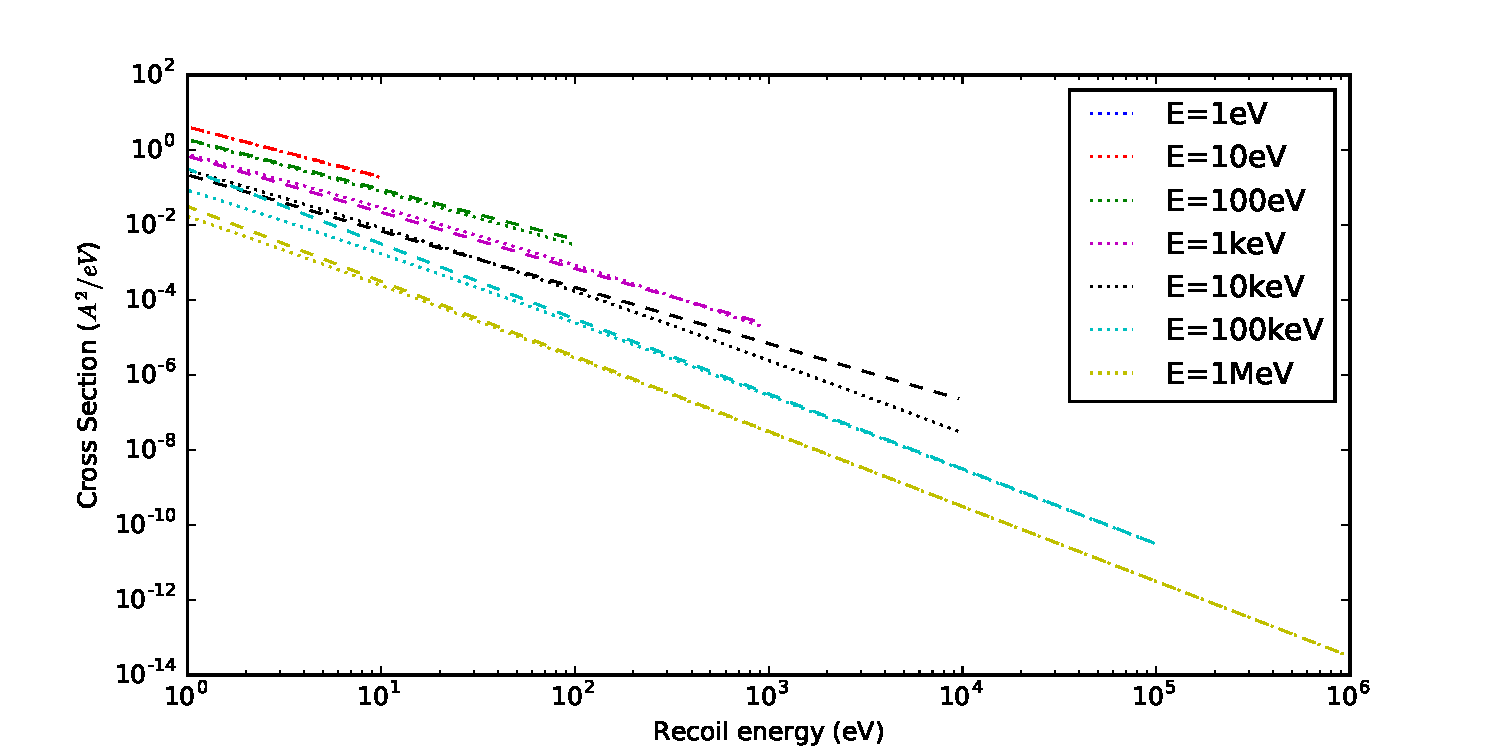
\includegraphics[width=1\linewidth]{thomas_fermi_vs_power.pdf}
	\caption{Cross sections obtained with the Thomas-Fermi (dotted) and power law potentials (dashed).}
	\label{fig:thomas_fermi_vs_power}
\end{figure}

\subsection{Numerical Solution of the Integrodifferential Equations}\label{sec:numerical_results}
In this section the numerical issues with solving Eqs.~\ref{eq:damage_energy_function_1},~\ref{eq:total_pc_1}, and ~\ref{eq:net_pc_1} are discussed. 
The major issue with solving these equations is that the interaction cross section is unbounded at $E \rightarrow 0$ and $T \rightarrow 0$. For Eq.~\ref{eq:damage_energy_function_1} all three terms on the right hand side need to be treated with care, while for Eqs. ~\ref{eq:total_pc_1} and ~\ref{eq:net_pc_1} only the last two terms cause problems because of the lower integration limit for the first term. We will start discussing the general numerical approach taken to integrate Eqs.~\ref{eq:damage_energy_function_1},~\ref{eq:total_pc_1}, and ~\ref{eq:net_pc_1} and then highlight the special treatment to ensure numerical stability.

Magpie uses algorithms implemented in the GNU scientific library (GSL)~\cite{GSL} for the solution of the relevant equations.The ODE is abstracted into the form
\begin{equation}\label{eq:general_ode}
   \frac{d \vec{x}}{dE} = \vec{F} \left( \vec{x},E \right),
\end{equation}
where $\vec{x}$ is a vector containing the unknowns $\nu_i$, $n_{i,j}$, or $g_{i,j}$. GSL provides functions to solve Eq.~\ref{eq:general_ode} given the ability to evaluate $\vec{F}$. Within this work, explicit stepping methods of the Runge-Kutta type are used and if not stated otherwise explicit 4th order (classical) Runge-Kutta (\textit{gsl\_odeiv2\_step\_rk4}) is used. Numerical integration of ODEs results in solution on an energy grid denoted by $E_l, l=1,..,L$ where the solution at these points is denoted by $\nu^{(l)}_i = \nu_i(E_l)$ (using the damage energy function as example).

The evaluation of $\vec{F}$ requires computing integrals over energy. Within work, we divide the range of integration over energy into a sum of integrals over the energy spacing between grid points:
\begin{equation}
  \int\limits_0^{\Lambda_{ik} E} \frac{d \sigma_{i,k}}{dT} f(E,T)  dT = \sum\limits_{l=1}^{L-1} \int\limits_{E_l}^{E_{l+1}}  \frac{d \sigma_{i,k}}{dT}f(E,T)  dT,
\end{equation}
where $f(E,T)$ is a placeholder for the damage energy or displacement function. 
The elementary integral on the right hand is estimated using GSL's Gauss-Legendre quadrature and  
he values of $f$ are interpolated linearly for energies between $E_l$ and $E_{l+1}$. If not stated otherwise a Gauss-Legendre quadrature of order $4$ is used.

The numerical difficulty with solving Eq.~\ref{eq:damage_energy_function_1} is that the cross section becomes unbounded if evaluated for small energies $E$ or $T$, in particular $ \frac{d \sigma_{i,k}}{dT} \propto E^{-1/3} T^{-4/3}$, while $\nu_k(T)$ and $\nu_i(E-T) - \nu_i(E)$ are asymptotically well represented by $c T$ where $c$ is independent of $T$ but may depend on $E$. Hence, for sufficiently small $E$, and consequently a small range of $T$, the terms on the right hand side behave as $T^{2/3} E^{-1/3}$. Numerical issues arise from separately evaluating the cross section and the damage energy function and then multiplying them to evaluate the integrand. 

For the solution of the damage energy equation Eq.~\ref{eq:damage_energy_function_1}  small values of $E$ we use the well known approximation for $\nu_i(E-T) - \nu_i(E)$ for small $T$~\cite{PC1980}:
\begin{equation}
   \nu_i(E-T) - \nu_i(E) \approx -T \frac{d\nu_i}{dE}.
\end{equation}
Substitution into Eq.~\ref{eq:damage_energy_function_1} and rearranging gives:
\begin{equation}\label{eq:damage_energy_function_approx_1}
    \frac{d \nu_i}{dE} 
      =\frac{ \sum\limits_{k=1}^K   \frac{N_k}{N} \int\limits_{0}^{\Lambda_{ik} E}  \frac{d \sigma_{ik} (E,T)}{dT}  
 \nu_k(T)  dT}{ S_i(E) +  \sum\limits_{k=1}^K   \frac{N_k}{N} \int\limits_{0}^{\Lambda_{ik} E} \frac{d \sigma_{ik} (E,T)}{dT}  T dT  },
\end{equation}
Finally, the term in the numerator is still problematic for $T << 1$. We define a threshold $E_t \approx 0.1$ eV and approximate $\nu_k(T) \approx T$ for $T < E_t$:
\begin{align}
 \int\limits_{0}^{\Lambda_{ik} E}  \frac{d \sigma_{ik} (E,T)}{dT}  &\approx  \int\limits_{0}^{\min(\Lambda_{ik} E, E_t)}  \frac{d \sigma_{ik} (E,T)}{dT} T dT
 \nonumber \\
      &+  H(\Lambda_{ik} E - E_t) \int\limits_{E_t}^{\Lambda_{ik} E}  \frac{d \sigma_{ik} (E,T)}{dT}   \nu_k(T)  dT,
\end{align}
where $H(x)$ is the Heaviside step function. The solution for 
\[
  \int\limits_{0}^{\min(\Lambda_{ik} E, E_t)}  \frac{d \sigma_{ik} (E,T)}{dT} T dT
\]
is obtained analytically using the low $t$ limit of the elastic scattering cross section given in Eq.~\ref{eq:thomas_fermi_lowt}.

For the solution of Eq.~\ref{eq:damage_energy_function_1} for large energies $E$, we still have to properly evaluate the integrals on the right hand side for small $T$. We use the same approach used for evaluating the denominator in Eq.~\ref{eq:damage_energy_function_approx_1}, namely splitting the integral at a lower threshold and then 
\begin{align}\label{eq:damage_energy_function_approx_2}
    \frac{d \nu_i}{dE}  & = \frac{1}{S_i(E)} \sum\limits_{k=1}^K   \frac{N_k}{N}  \nonumber \\
                                 & \times \left [     
     \int\limits_{0}^{\min(\Lambda_{ik} E, E_t)}  \frac{d \sigma_{ik} (E,T)}{dT} T dT
 +  H(\Lambda_{ik} E - E_t) \int\limits_{E_t}^{\Lambda_{ik} E}  \frac{d \sigma_{ik} (E,T)}{dT}   \nu_k(T)  dT
        \right . \nonumber \\ 
     & - \frac{d \nu_i}{dE }   \int\limits_{0}^{\min(\Lambda_{ik} E, E_t)}  \frac{d \sigma_{ik} (E,T)}{dT} T dT \nonumber \\
       &   \left .      + H(\Lambda_{ik} E - E_t) \int\limits_{E_t}^{\Lambda_{ik} E}  \frac{d \sigma_{ik} (E,T)}{dT}  \left( \nu_i(E-T) - \nu_i(E) \right)  dT  \right ], 
\end{align}
where the derivative $\frac{d \nu_i}{dE}$ is approximated using a backward finite difference:
\begin{equation}
   \frac{d \nu_i}{dE} \approx \frac{\nu_i^{(L)} - \nu_i^{(L-1)}}{E_L - E_{L-1}}.
\end{equation}

The total and net displacement rates do not suffer from problems when integrating to small $E$ as initial conditions are given at an energy of the order of $10$ eV. In addition, the first integral on the right hand side does not suffer from problems with evaluating the integrand at small energies because the displacement probability essentially translates into a sufficiently larger lower integration limit. The second and third integrals suffer from the same problem as the damage energy function and the applied treatment is identical to the one outlined in Eq.~\ref{eq:damage_energy_function_approx_2}.

\subsection{Comparison of Results with Literature (and Other Codes)}
Results obtained with the described implementation are compared with polyatomic damage energy functions reported in Ref.~\cite{PC1980} and damage efficiencies $k_{i,j}$ reported in Ref.~\cite{PC1981}. The damage efficiency $k_{i,j}$ is defined by:
\begin{equation}
   k_{i,j}(E)  =\frac{\left( g_{i,j}(E) - \delta_{i,j} \right) E_j^d}{f_j \nu_i(E)}.
\end{equation}
We compare the damage energy functions for $\text{Al}_2\text{O}_3$, $\text{U}_x\text{Zr}_{1-x}\text{C}$ for $x=0.02, 0.5, 0.98$, and the damage efficiencies for $\text{Al}_2\text{O}_3$, TaO, and UC.

The damage energy functions computed with Magpie for  $\text{Al}_2\text{O}_3$ are compared with~\cite{PC1980} in Table~\ref{tab:Al2O3_energy}.
The discrepancy between Parkin and Coulter's results and Magpie are between $5$ and $40$ \% and tends to be highest for intermediate values of energy at $10$ keV. While this difference appears large it should be pointed out that Parkin and Coulter and Magpie use different cross section and stopping power relations that may explain the difference. Reference~\cite{PC1980} states that using the Winterborn, Sigmund and Sanders approximaton to the universal scattering function leads to an overestimation of the damage energy function. In addition, we use \textit{mytrim} stopping power relations, while Parkin and Coulter use Lindhard's stopping power formula~\cite{Lindhard1963}. If these differences cause the differences in the damage energy function of $\text{Al}_2\text{O}_3$ cannot be determined with certainty without more investigation. However, the difference are within acceptable limits within the field of radiation damage estimation. 

\begin{table}[p]
  \centering
  \caption{Comparison of damage energy function for  $\text{Al}_2\text{O}_3$ computed with Magpie and reported in~\cite{PC1980}. \label{tab:Al2O3_energy}}
\begin{tabular}{l*{6}{c}}
Energy (eV)              & Ref. Al & Al & Rel. Diff (\%) & Ref. O & O & Rel. Diff (\%) \\
\hline
   $10^1$ &     0.87 &     0.95 &     8.82 &     0.86 &     0.93 &     7.66 \\
  $10^2$ &     0.83 &     0.91 &    10.49 &     0.82 &     0.89 &     8.98 \\
 $10^3$ &     0.77 &     0.91 &    18.02 &     0.75 &     0.88 &    18.33 \\
 $10^4$ &     0.69 &     0.87 &    26.98 &     0.61 &     0.78 &    28.87 \\
$10^5$ &     0.50 &     0.68 &    36.40 &     0.31 &     0.42 &    34.93 \\
$10^6$ &     0.17 &     0.22 &    32.41 &     0.07 &     0.09 &    28.00 \\
$10^7$ &     0.02 &     0.03 &    27.05 &     0.01 &     0.01 &    27.96 \\
\hline
\end{tabular}
\end{table}

The damage energy functions for  $\text{U}_x\text{Zr}_{1-x}\text{C}$ for $x=0.02, 0.5, 0.98$ computed by Magpie are reported in Table~\ref{tab:UZrC_energy}; comparison with the results reported in
Ref.~\cite{PC1980} is provided in Table~\ref{tab:UZrC_energy_comparison}. Differences between Magpie and Parkin and Coulter's results are on the same order of magnitude as for $\text{Al}_2\text{O}_3$ for higher energies but are much smaller for low,  $E<1$ keV and intermediate energies, $~10keV$. Magpie qualitatively reproduces the trends discussed in~\ref{PC1980}
when changing $x$ for all species correctly. Magpie agrees well with the reference for uranium and zirconium at low energies but overestimates them at higher energies, while consistently underestimating carbon. 

\begin{table}[p]
  \centering
  \caption{Damage energy function for  $\text{U}_x\text{Zr}_{1-x}\text{C}$ for three different values of $x_=0.02, 0.5, 0.98$  denoted by $x_i,~i=1,..,3$ computed with Magpie. \label{tab:UZrC_energy}}
\begin{tabular}{c c c c c c c c c c}
         & \multicolumn{3}{c}{U} & \multicolumn{3}{c}{Zr} & \multicolumn{3}{c}{C} \\
         \cline{2-4} \cline{5-7} \cline{7-10}
Energy (eV)              & $x_1$& $x_2$& $x_3$& $x_1$&$x_2$ &$x_3$ &$x_1$&$x_2$ &$x_3$\\
\hline
   $11.2$ &     0.89 &     0.89 &     0.89 &     0.89 &     0.88 &     0.88 &     0.74 &     0.72 &     0.69 \\
  $107$ &     0.84 &     0.84 &     0.84 &     0.83 &     0.82 &     0.82 &     0.66 &     0.64 &     0.60 \\
 $1020$ &     0.81 &     0.81 &     0.81 &     0.79 &     0.78 &     0.78 &     0.60 &     0.57 &     0.54 \\
$1.15 \times 10^4$ &     0.75 &     0.75 &     0.76 &     0.73 &     0.72 &     0.72 &     0.44 &     0.41 &     0.39 \\
$1.1 \times 10^5$ &     0.67 &     0.67 &     0.68 &     0.64 &     0.64 &     0.65 &     0.19 &     0.19 &     0.19 \\
$1.05 \times 10^6$ &     0.54 &     0.56 &     0.57 &     0.47 &     0.50 &     0.52 &     0.04 &     0.04 &     0.04 \\
$10^7$ &     0.30 &     0.33 &     0.36 &     0.16 &     0.19 &     0.21 &     0.01 &     0.01 &     0.01 \\
\hline
\end{tabular}
\end{table}

\begin{table}[p]
  \centering
  \caption{Relative difference of damage energy functions for  $\text{U}_x\text{Zr}_{1-x}\text{C}$ for three different values of $x_=0.02, 0.5, 0.98$  denoted by $x_i,~i=1,..,3$ between Magpie and results reported in~\cite{PC1980}. \label{tab:UZrC_energy_comparison}}
\begin{tabular}{c c c c c c c c c c}
         & \multicolumn{3}{c}{U} & \multicolumn{3}{c}{Zr} & \multicolumn{3}{c}{C} \\
         \cline{2-4} \cline{5-7} \cline{7-10}
Energy (eV)              & $x_1$& $x_2$& $x_3$& $x_1$&$x_2$ &$x_3$ &$x_1$&$x_2$ &$x_3$\\
\hline
   $11.2$ &     0.07 &     0.64 &     1.00 &     1.10 &     1.55 &     1.85 &     9.87 &     9.85 &    10.01 \\
   $107$ &     1.93 &     1.14 &     0.70 &     0.86 &     0.22 &     0.33 &    12.87 &    12.95 &    13.27 \\
 $1020$ &     0.71 &     1.52 &     2.29 &     1.63 &     2.68 &     3.69 &    11.25 &    10.82 &    10.71 \\
$1.15 \times 10^4$ &     2.40 &     3.90 &     4.94 &     4.54 &     6.43 &     7.98 &    14.07 &    12.38 &    10.91 \\
$1.1 \times 10^5$ &     5.04 &     6.90 &     8.26 &    10.29 &    13.04 &    15.47 &    21.02 &    16.63 &    12.29 \\
$1.05 \times 10^6$ &     9.08 &    11.39 &    12.72 &    22.65 &    28.38 &    32.52 &    26.26 &    22.87 &    19.15 \\
$10^7$ &     7.42 &    12.58 &    15.73 &    27.05 &    36.70 &    44.03 &    23.95 &    17.27 &    21.79 \\
\hline
\end{tabular}
\end{table}

The comparison of Parkin and Coulter's damage efficiencies and computed Magpie results for  $\text{Al}_2\text{O}_3$ are shown in Fig.~\ref{fig:kij_Al2O3}. Within this work we use set the capture energies to $E_{i,j}^{\text{cap}} = (18, 45, 45, 72)$. Damage efficiences follow the same trend 
and agree well when judged in proportion to each other:
\begin{itemize}
  \item For both Magpie and PC's results the Al-Al and O-Al as well as the Al-O and O-O damage energy functions are very similar for large energies. 
  \item The Al-Al and O-Al damage efficiences are larger than the O-Al and O-O damage energies by roughly the same amount for Magpie and the reference's results. 
\end{itemize}
The significant difference is the overestimation of the reported damage efficiencies by $5$ \%.

\begin{figure}[p]
	\centering
	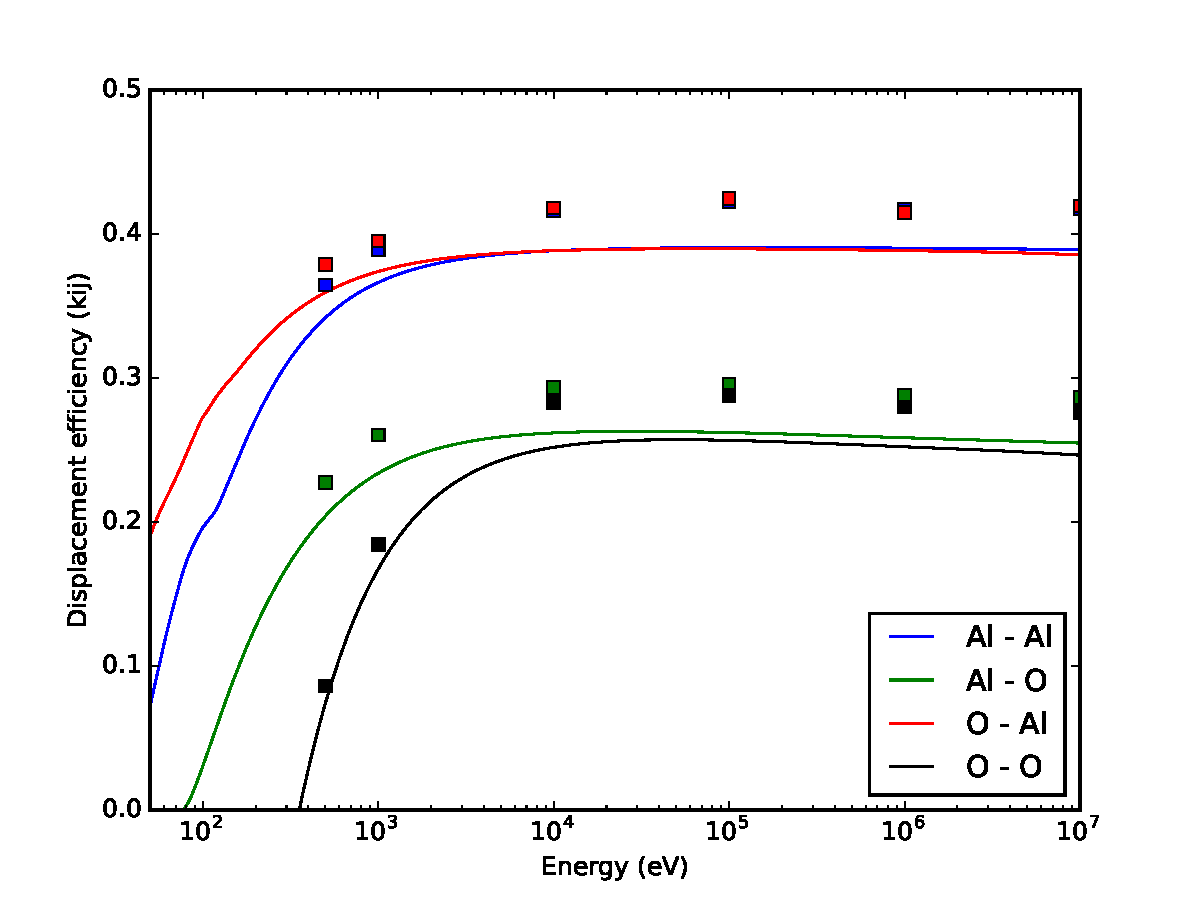
\includegraphics[width=1\linewidth]{comparison_parkin_coulter_Al2O3/comparison_PC_1981_Magpie_Al2O3.pdf}
	\caption{Damage efficiencies for $\text{Al}_2\text{O}_3$ computed by Magpie (solid lines) and from Ref~\cite{PC1981} (square markers).}
	\label{fig:kij_Al2O3}
\end{figure}

Magpie is used to compute the displacement efficiency of TaO using $E_{i,j}^{\text{cap}}=(60,60,60,60)$ and the comparison with results in Ref.~\cite{PC1981} is shown in Fig.~\ref{fig:kij_TaO} where Magpie results are represented by solid lines and results by PC are represented by dashed lines. Magpie reproduces the trends reported by Parkin and Coulter but consistently underestimates the reported results by $0.05$ to $0.1$.
\begin{figure}[p]
	\centering
	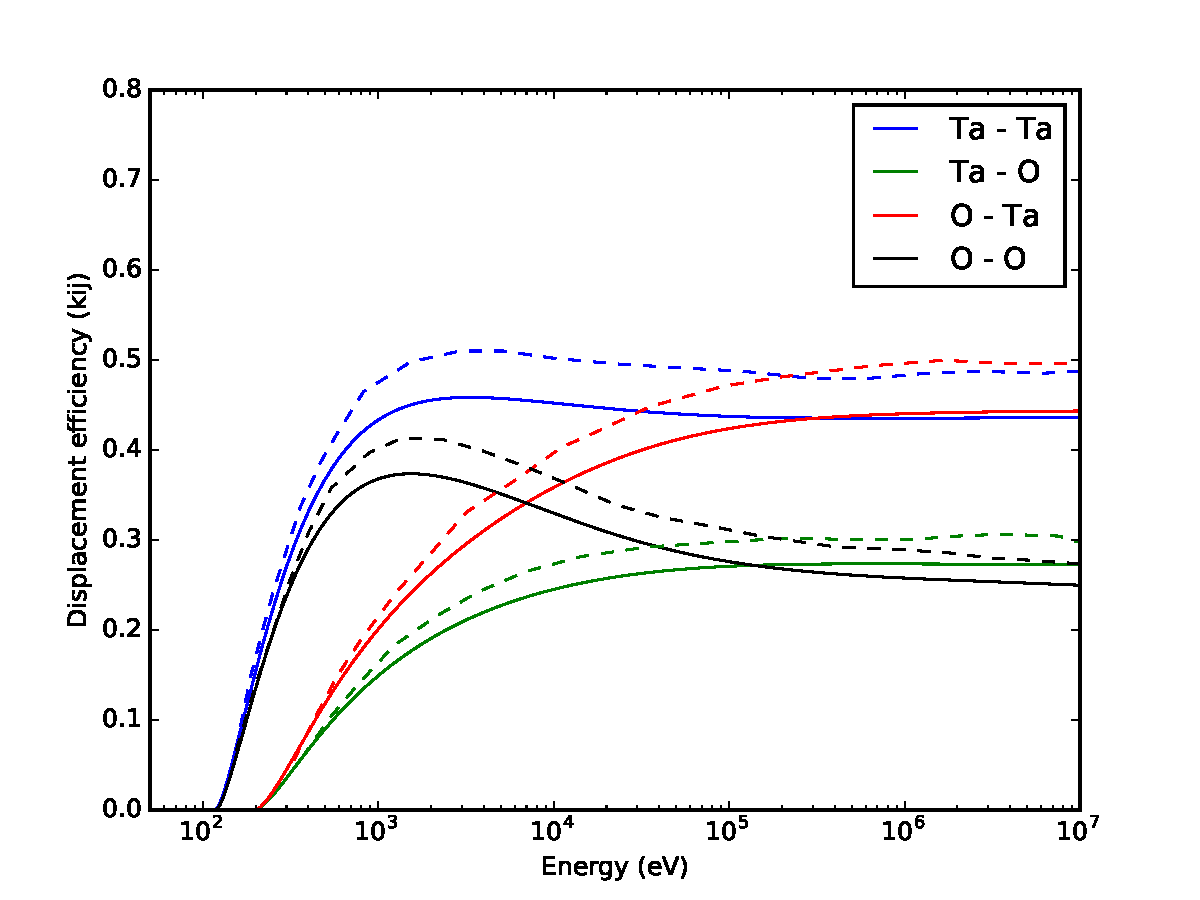
\includegraphics[width=1\linewidth]{comparison_parkin_coulter_TaO/comparison_PC_1981_Magpie_TaO.pdf}
	\caption{Damage efficiencies for TaO computed by Magpie (solid lines) and from Ref~\cite{PC1981} (dashed lines).}
	\label{fig:kij_TaO}
\end{figure}

Finally, damage efficiencies of UC are compared with Parkin and Coulter's result at $E=10^{7}$ eV in Table~\ref{tab:UC_kij}. Magpie and PC's results are in excellent agreement with relative differences well below $10$ \%.

\begin{table}[p]
  \centering
  \caption{Comparison of displacement efficiencies $k_{i,j}$ for UC for different threshold energy values computed by Magpie and reported in Ref.~\cite{PC1980}. $k_{i,j}$ denotes the values computed by Magpie and Diff denotes the relative difference between the Magpie result and the value reported by Parkin and Coulter in \% \label{tab:UC_kij}}
\begin{tabular}{c c c c c c c c c}
   & \multicolumn{2}{c}{U-U}& \multicolumn{2}{c}{U-C}&\multicolumn{2}{c}{C-U} & \multicolumn{2}{c}{C-C} \\  
   \cline{2-9}
   $E_{i,j}^{\text{cap}}$ & $k_{i,j}$& Diff  & $k_{i,j}$& Diff & $k_{i,j}$& Diff & $k_{i,j}$& Diff \\ 
\hline
 (1,1,1,1)         & 0.485& 6.9 &   0.262 & 1.4 & 0.490 & 6.2&  0.255 & 1.2\\
 (60,60,60,60) & 0.575 & 5.5 &  0.237  &0.1 & 0.573 &4.5 &  0.208 & 1.7\\
 (10,60,60,60) & 0.530  &6.5 &  0.228  &1 & 0.536 & 5.6 & 0.200&0.6 \\
 (60,60,60,10) & 0.553  &4 &  0.256 &2.1 &  0.550 &2.8 &  0.238& 1.0\\
\hline
\end{tabular}
\end{table}
\clearpage

\subsubsection{Perturbation Theory Approach}
In this section, we derive an equation for the derivative of the net displacement function with respect to the $l$-th number fraction, i.e. $\theta_{ijl} \equiv \frac{d g_{ij}}{d f_l}$, where $f_l = N_l / N$. The purpose of computing the derivative is to estimate the changes of the net displacement function when the number fractions change. To first order, changing the number densities $f_l$ to $f_l'$ lead to the following changes in the net displacement rates:
\begin{equation}\label{eq:first_order_net}
   g_{ij} (E,\vec{f}') =  g_{ij} (E,\vec{f}) + \sum\limits_{l=1}^K \theta_{ijl}(E,\vec{f}) (f_l' - f_l).  
\end{equation}

The equations describing the derivative of the net displacement with respect to number fractions is derived using first order perturbation theory. We first introduce a small perturbation $\delta f_l$ that causes a small perturbation in the net displacement function denoted by $\delta g_{ij}^{(l)}$. The perturbation of $f_l$ is chosen to be small enough so that products of two perturbations can be neglected; in the remainder of this work, these terms are referred to as higher order terms. Substituting:
\begin{align}
   f_k & \leftarrow f_k + \delta f_l ~\delta_{l,k} \nonumber \\
    g_{ij} & \leftarrow g_{ij} + \delta g_{ij}^{(l)} \nonumber \\
    s_i & \leftarrow s_i +\delta s_i^{(l)},
\end{align}
into Eq.~\ref{eq:net_pc_1} leads to:
\begin{align}
 \left(s_i(E) + \delta s_i \right)&\left[ \frac{d g_{ij}}{dE} + \frac{d \delta g_{ij}^{(l)}}{dE} \right] = \sum\limits_{k=1}^K \left( f_k + \delta f_l \delta_{l,k}  \right)
  \int\limits_0^{\Lambda_{ik}E} dT \frac{d \sigma_{ik}}{dT}  \times
 \nonumber \\
 &\times \left \{ \rho_k(T) \left[ g_{kj}(T-E_k^b) + \delta g^{(l)}_{kj}(T-E_k^b)  \right] \right . \nonumber \\
 &+ (1 - \rho_k(T) \lambda_{ik}(E-T) ) \left[ g_{ij}(E-T) + \delta g^{(l)}_{ij}(E-T) \right]  \nonumber \\
 & \left . - \left[  g_{ij}(E) + \delta g^{(l)}_{ij}(E) \right]   \right\}.
\end{align}
We now multiply out the parentheses and neglect all terms of order higher than one:
\begin{align}
 &s_i(E) \frac{d g_{ij}}{dE} + \delta s_i(E)  \frac{d (\delta g_{ij})}{dE}  +  s_i(E)\frac{d \delta g_{ij}^{(l)}}{dE} 
   = \sum\limits_{k=1}^K \int\limits_{0}^{\Lambda_{ik} E} dT \frac{d \sigma_{ik}}{dT} \Bigg [ 
 \nonumber \\
 & f_k \left (  \rho_k(T) g_{kj}(T-E_k^b)   + (1 - \rho_k(T) \lambda_{ik}(E-T) ) g_{ij}(E-T)  - g_{ij}(E) \right ) \nonumber \\
 +& f_k \left (  \rho_k(T) \delta g_{kj}^{(l)}(T-E_k^b)   + (1 - \rho_k(T) \lambda_{ik}(E-T) ) \delta g_{ij}^{(l)}(E-T)  - \delta g_{ij}^{(l)}(E) \right ) \nonumber \\
 +&\delta   f_k \delta_{l,k} \left (  \rho_k(T) g_{kj}(T-E_k^b)   + (1 - \rho_k(T) \lambda_{ik}(E-T) ) g_{ij}(E-T)  - g_{ij}(E) \right ) \Bigg ].
\end{align}
Using the original, unperturbed equation for the net displacement, we can cancel several terms:
\begin{align}\label{eq:net_disp_pert_0}
& \delta s_i(E)  \frac{d g_{ij}}{dE}  +  s_i(E)\frac{d (\delta g_{ij}^{(l)})}{dE} 
   = \sum\limits_{k=1}^K  f_k \int\limits_{0}^{\Lambda_{ik} E} dT \frac{d \sigma_{ik}}{dT} \Bigg [   \rho_k(T) \delta g_{kj}^{(l)}(T-E_k^b)   
 \nonumber \\
 +& (1 - \rho_k(T) \lambda_{ik}(E-T) ) \delta g_{ij}^{(l)}(E-T)  - \delta g_{ij}^{(l)}(E) \Bigg ] \nonumber \\
 +&\delta   f_l   \int\limits_{0}^{\Lambda_{il} E} dT \frac{d \sigma_{il}}{dT} \Bigg [  \rho_l(T) g_{lj}(T-E_l^b)   + (1 - \rho_l(T) \lambda_{il}(E-T) ) g_{ij}(E-T)  - g_{ij}(E) \Bigg ] .
\end{align}
Now Eq.~\ref{eq:net_disp_pert_1} is divided by $\delta f_l$:
\begin{align}\label{eq:net_disp_pert_1}
& \frac{\delta s_i(E)}{\delta f_l}  \frac{d g_{ij}}{dE}  +  s_i(E)\frac{d}{dE} \left( \frac{ \delta g_{ij}^{(l)}}{\delta f_l} \right) 
   = \sum\limits_{k=1}^K  f_k \int\limits_{0}^{\Lambda_{ik} E} dT \frac{d \sigma_{ik}}{dT} \Bigg [   \rho_k(T)   \frac{\delta g_{kj}^{(l)}}{\delta f_l}(T-E_k^b)   
 \nonumber \\
 +& (1 - \rho_k(T) \lambda_{ik}(E-T) ) \frac{\delta g_{ij}^{(l)}}{{\delta f_l}}(E-T)  - \frac{\delta g_{ij}^{(l)}}{{\delta f_l}}(E) \Bigg ] \nonumber \\
 +&  \int\limits_{0}^{\Lambda_{il} E} dT \frac{d \sigma_{il}}{dT} \Bigg [  \rho_l(T) g_{lj}(T-E_l^b)   + (1 - \rho_l(T) \lambda_{il}(E-T) ) g_{ij}(E-T)  - g_{ij}(E) \Bigg ] .
\end{align}
By passing to the limit $\delta f_l \rightarrow 0$ we can write the following fractions as derivatives:
\begin{align}
  \lim\limits_{\delta f_l \rightarrow 0} \frac{ \delta g_{ij}^{(l)}}{\delta f_l} = \frac{d g_{ij}}{d f_l} = \theta_{ijl} \nonumber \\
  \lim\limits_{\delta f_l \rightarrow 0} \frac{\delta s_i(E)}{\delta f_l} = \frac{d s_i}{d f_l}
\end{align}
Substitution into Eq.~\ref{eq:net_disp_pert_1} provides an equation for $\theta_{ijl}$:
\begin{align}\label{eq:net_disp_pert_final}
&   s_i(E)\frac{d \theta_{ijl}}{dE}  
   = \sum\limits_{k=1}^K  f_k \int\limits_{0}^{\Lambda_{ik} E} dT \frac{d \sigma_{ik}}{dT} \Bigg [   \rho_k(T) \theta_{kjl}(T-E_k^b)   
 \nonumber \\
 +& (1 - \rho_k(T) \lambda_{ik}(E-T) )  \theta_{ijl}(E-T)  -\theta_{ijl}(E) \Bigg ]  + S_{i,j,l}(E)\nonumber \\
 S_{i,j,l}(E)=&  \int\limits_{0}^{\Lambda_{il} E} dT \frac{d \sigma_{il}}{dT} \Bigg [  \rho_l(T) g_{lj}(T-E_l^b)    \nonumber \\ 
 +& (1 - \rho_l(T) \lambda_{il}(E-T) ) g_{ij}(E-T)  - g_{ij}(E) \Bigg ] \nonumber \\
 -& \frac{ds_i(E)}{d f_l}  \frac{d g_{ij}}{dE}.
\end{align}
The initial conditions for the net displacement rates are $g_{ij}(E) = \delta_{ij} \text{ for } E< \min\limits_{i} (E_i^d)$ which are independent of $f_l$. Therefore, the initial condition for $\theta_{ijl}$ is $\theta_{ijl}(E) = 0 \text{ for } E< \min\limits_{i} (E_i^d)$. Equation~\ref{eq:net_disp_pert_final} looks  similar to the original equation for the net displacement function, Eq.~\ref{eq:net_pc_1}, except for the source term $S_{i,j,l}$. Therefore, solution is straight forward by first obtaining $g_{ij}$ and then using the same algorithm for computing $\theta_{ijl}$ with the only difference that $S_{ijl}$ is computed from the computed net displacement rate and then added to the right hand side.

We test the correct implementation using the $\text{Al}_2\text{O}_3$ example described in section~\ref{sec:numerical_results}. A base case calculation is performed using number fractions of $0.4$ and $0.6$ for Al and O, respectively; then the number fractions are modified to $0.3$ and $0.7$, respectively, corresponding to $\delta f_{\text{Al}} = -0.1$ and $\delta f_{\text{O}} = 0.1$.  The net displacement rates are then (1) re-computed using the new number fractions and (2) estimated to first order using Eq.~\ref{eq:first_order_net}. The results are presented in Fig.~\ref{fig:fop_Al2O3}. The markers indicate the direct computation of $g_{ij}$ with modified number fractions, while the dashed-dotted line indicates the estimation using first order perturbation (fop) theory. We observe that estimated and directly computed values agree very well. 

\begin{figure}[p]
	\centering
	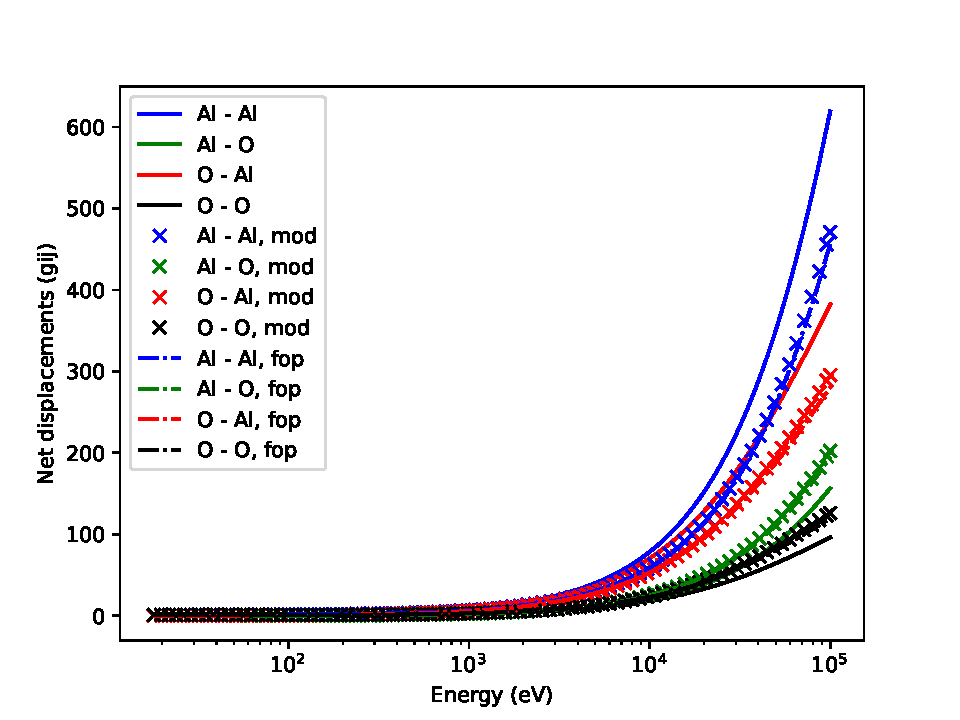
\includegraphics[width=1\linewidth]{comparison_parkin_coulter_Al2O3_first_order_perturbation/NRT_first_order_perturbation_theory.pdf}
	\caption{Testing the correctness and precision of estimating the change in net displacement rates of $\text{Al}_2\text{O}_3$ due to changes in number fractions using first order perturbation theory. The solid lines represent $g_{ij}$ for the base number fractions $0.4$/$0.6$, the markers indicate direct computation of the modified system with number fractions $0.3$/$0.7$, the dashed-dotted lines indicate the estimation using first order perturbation theory.}
	\label{fig:fop_Al2O3}
\end{figure}

\subsection{Deployment of Polyatomic NRT Model in Magpie}
The polyatomic NRT model is used in Magpie to shorten damage cascades if the recoil energy drops below a threshold $E_t$. The condition for NRT to be applicable is that the recoil that is currently being simulated on its random walk is 
represented in the list of matrix species. If the recoil is a matrix atom, it can be treated using the polyatomic NRT method, otherwise its random walk is completed using MYTRIM only. 

We do not compute NRT damage functions $g_{ij}$ per mesh element but cache existing damage functions by their composition vector $\vec{f}_q$, where the subscript $q$ indicates that the cached damage functions is the $q$-th damage functions, where $q=1,..,Q$; we denote the $q$-th damage function as $g^{(q)}_{ij}$ and its derivative with respect to number fraction $l$ as $\theta^{(q)}_{ijl}$. For the first recoil whose energy drops below $E_t$, no damage functions exists, so $g^{(1)}_{ij}$ and $\theta^{(1)}_{ijl}$ are computed at the composition that the recoil experiences its first collision with energy $E < E_t$. For subsequent recoils with $E<E_t$ we determine the damage functions and its derivative that is computed at a composition that most closely matches the current composition $\vec{f}$:
\begin{equation}
 q^* = \argmin\limits_{q=1,...,Q} \| \vec{f} -\vec{f}_q \|_{\infty}.
\end{equation}
The cached damage function is used if $ \| \vec{f} -\vec{f}_{q^*} \|_{\infty} < \epsilon$, where $\epsilon$ is a user supplied tolerance usually set to $\epsilon = 0.25$. 
If $ \| \vec{f} -\vec{f}_q \|_{\infty} > \epsilon$, a new damage function is computed for composition $\vec{f}$ and added to the set of existing damage functions. The value of the net displacement function $g_{ij}^{(q^*)}(E, \vec{f}) $ is then computed at energy $E$ for all targets $j=1,...,K$ using Eq.~\ref{eq:first_order_net}. The locally deposited energy is incremented by $g_{ij}^{(q^*)}(E, \vec{f}) E_j^b$, and entries in the interstitial and vacancy site vectors with weight $g_{ij}^{(q^*)}(E, \vec{f})$ are created. The recoil is then removed from the queue of recoils. 

Tests and results to come...

\subsubsection{Computation of Damage Cross Sections}
to come...
%**********************************************************************************************************************************************************************************************%

%\section*{References}
\clearpage
\section*{References}
\bibliography{bibdata}

\end{document}